\documentclass[11pt,a4paper,openany,leqno]{article}

\textwidth=160mm \textheight=260mm \hoffset=-18mm \voffset=-30mm
\setcounter{page}{1}
			\usepackage[magyar]{babel}
			\usepackage[utf8]{inputenc}
			\usepackage[T1]{fontenc}
			\usepackage{indentfirst}
			\usepackage{amsmath,esint}
			\usepackage{amssymb}
%			\usepackage{eufrak}
			\usepackage{psfrag}
			\usepackage{tabularx}
			\usepackage{graphicx}
			\usepackage{wrapfig}	
			\usepackage{hyperref}
			\usepackage{multicol}	
									
			\frenchspacing
			\allowhyphens

\tolerance=2000
\hbadness=2000
\vbadness=10000
\overfullrule=0pt




\begin{document}
\section{Indukció II.}
\subsection{Elméleti Fizikai Példatár II. / 6.22. feladat}
Hosszú egyenes vezető és $a$ sugarú gyűrű egy síkban fekszik. A gyűrű középpontjának a vezetőtől mért távolsága $b$ ($b>a$). Határozzuk meg az $L_{12}$ kölcsönös indukciós együtthatót és az $F_{12}$ kölcsönhatási erőt, ha az áram az egyenes vezetőben $I_1$ és a gyűrűben $I_2$.

 \indent


\begin{figure}[h!]
\centering
  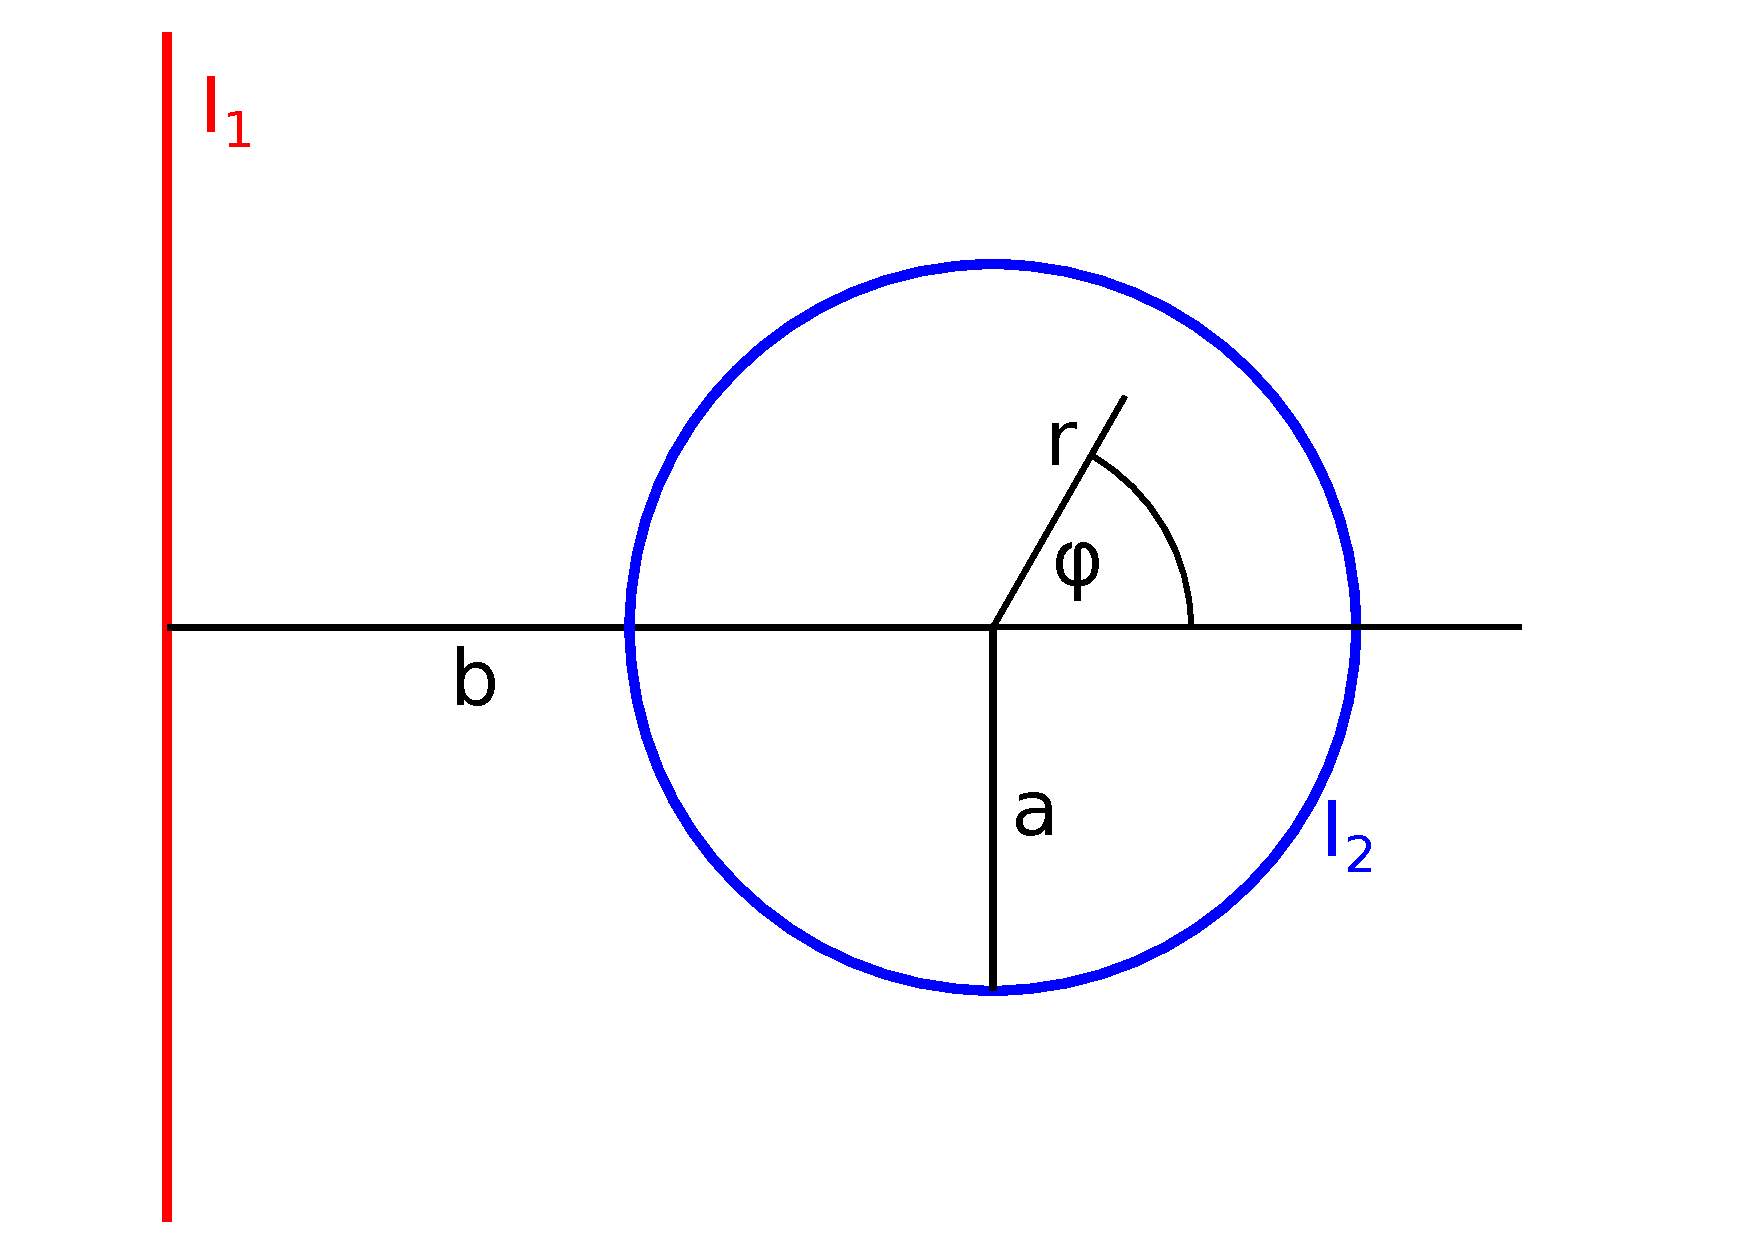
\includegraphics[width=120mm,scale=0.5]{kep.pdf}
  \caption{A hosszú egyenes vezető és a gyűrű}
  \label{}
\end{figure} 


\begin{flushright} {Feladatot kidolgozta: {\it Z2R8XS}} \end{flushright}

\vspace{0.5cm}

\textbf{Megoldás}\\
\indent
Tudjuk, hogy a végtelen hosszú vezető mágneses terének erőssége a vezetőtől $r$ távolságban\\
$$ B(\varrho) = \frac{\mu_0 \cdot I}{2\cdot \pi \cdot \varrho} $$\indent
ahol $I$ a vezetőben folyó áram erőssége.\\ \indent
A kölcsönös indukciós együttható kiszámolható a fluxus és a vizsgált teret létrehozó áram erősségével.\\
$$ \Phi_{12} = I_1 \cdot L_{12} $$
$$ L_{12} = \frac{\Phi_{12}}{I_1} $$
A körvezetőre célszerű sík zsáktartományt húzni, mert egyéb esetben csak nehezítené az integrálást. Ez a kört leképezhető egy $(\phi,r)$ paramétertartományra, ahol elvégezhető az integrálás.\\ \indent
Az integrálás előtt még kifejezendő a mágneses tér erősségének helyfüggése a körvezető középpontjához rögzített polárkoordinátákkal.\\ \indent
$$ \varrho = b + r\cdot cos(\phi) $$\indent
Tudjuk, hogy $dx\cdot dy = r\cdot dr \cdot d\phi$
$$ L_{12} = \frac{1}{I_1} \int_{0}^{2\pi} d\phi \int_{0}^{a}dr (\frac{\mu_0 \cdot I_1 \cdot r}{2\cdot \pi \cdot(b+r\cdot cos(\phi)})) $$
$$ L_{12} = \frac{\mu_0}{2\cdot \pi} \int_{0}^{2\pi} d\phi \int_{0}^{a}dr (\frac{r}{b+r\cdot cos(\phi)}) $$
$$ L_{12} = \frac{\mu_0}{2\cdot \pi} \int_{0}^{a}dr \frac{2\cdot \pi \cdot r}{\sqrt{b^2 - r^2}} $$
$$ L_{12} = \frac{\mu_0}{2\cdot \pi} \int_{0}^{a}dr \frac{2\cdot \pi \cdot r}{\sqrt{b^2 - r^2}} $$
$$ L_{12} = \mu_0\cdot(b-\sqrt{b^2 - a^2}) $$
\indent
Az intuktivitás energiája\\
$$ W = \frac{1}{2}L_{12}\cdot I_1\cdot I_2 + \frac{1}{2}L_{21}\cdot I_2\cdot I_1 $$\indent
A kölcsönös indukciós együtthatóról tudni, hogy $L_{12} = L_{21}$, így\\
$$ W = L_{12}\cdot I_1\cdot I_2 $$\indent
Érezhető, hogy a kölcsönhatási erő a körvezető középpontját a hosszú vezetőre merőlegesen leképező egyenes mentén fog hatni, legyen ez egy "$b$ irány". A Lorentz erő a körvezetőben mindenhol radiális irányban fog mutatni. A rendszernek a vezetővel párhuzamos irányú eltolási szimmetriája van. Két azonos távolságra lévő pontban ható erő $b$ irányra merőleges komponense nem ad járulékot az eredő erőbe, ezek a $b$-re merőleges komponensek kiejtik egymást. Maradnak a $b$ irányú komponensek. A távolabb lévő pontokra kisebb, a közelebb lévők nagyobb erő hat. Az erők iránya, azaz hogy radiálisan kifelé vagy belefelé mutatnak-e, $I_1$ és $I_2$ áramok irányától függnek. Az erő nagyságának meghatározásához ezt nem szükséges tudni.\\ \indent
Fixáljuk, hogy egy $a$ sugarú körvezetőről beszélünk. A körvezető $b$ irányú eltolásához munkát kell végeznünk. A munkával megváltoztatjuk az induktivitási energiát. Rögzített sugár mellett $W$ felfogható, mint egy $V$ potenciális energia, mely csak $b$-től függ. \\ \indent
Az erő ekkor a potenciális energia negatív gradiense. A gradiens itt egy dimenziós mozgásra vonatkozik, tehát$ \nabla = \partial _b$.\\
$$ |\vec{F}_{12}| = F_{12} = -\nabla W = \frac{-\partial }{\partial b}W $$
$$ F_{12} = \frac{-\partial }{\partial b}(\mu_0\cdot I_1 \cdot I_2 \cdot (b-\sqrt{b^2 - a^2})) $$
$$ F_{12} = -\mu_0\cdot I_1 \cdot I_2 \cdot (\frac{b}{\sqrt{b^2 - a^2}}+1)) $$
$$ |F_{12}| = \mu_0\cdot I_1 \cdot I_2 \cdot (\frac{b}{\sqrt{b^2 - a^2}}+1)) $$



\end{document}